%=
%=
%=
%=
%=
%=
\chapter{Sismologie et imagerie de la Terre}\label{ch:b3:seismology-imaging}

Le 22 mai 1960, à 19:11 temps universel, le plus fort séisme enregistré depuis
1900 a rompu la zone de subduction au large du sud du Chili, avec une magnitude de 9.5.
% ledger: usgs5:chile1960
Ses ondes P atteignirent des stations situées de l'autre côté de la planète environ vingt minutes
plus tard~; ses ondes de surface firent plusieurs fois le tour du globe~; et pendant des jours
ensuite, les instruments les plus lents enregistrèrent toute la Terre en train de vibrer avec
des périodes voisines d'une heure, comme une cloche frappée. Chacun de ces signaux porte
des informations sur les roches qu'il a traversées. À partir des temps d'arrivée de millions de
telles ondes, relevées à des milliers de stations, les sismologues ont construit non seulement
le modèle stratifié de la Terre rappelé plus bas, mais aussi des images tridimensionnelles de
le manteau, où des panneaux plongeants et des panaches ascendants apparaissent comme des zones où
les ondes se propagent un peu plus vite ou un peu plus lentement que la moyenne. Ce chapitre montre comment~:
comment les rais se propagent dans une Terre sphérique, comment les ondes de surface sondent la croûte
et le manteau grâce à leur dispersion, comment les oscillations libres de l'ensemble de la
planète sont décrites, et comment quelques milliers de temps de trajet sont transformés en une
image par la résolution d'un \omterm{def:b3:seismology-imaging:inverse}{problème inverse} linéaire.

\begin{recall}
Dans un solide élastique isotrope se propagent deux types d'ondes de volume~: les ondes P, à la
vitesse $\alpha = \sqrt{(K + \tfrac43\mu)/\rho}$, et les ondes S, à la
vitesse $\beta = \sqrt{\mu/\rho}$, où $K$ et $\mu$ sont les modules d'incompressibilité et de cisaillement
et $\rho$ la masse volumique~; les ondes S ne se propagent pas dans un liquide (le volume de physique
de troisième année, au chapitre sur l'élasticité des milieux continus). Une onde dont la vitesse de phase
dépend de sa fréquence est dispersive~; son énergie se propage à la
vitesse de groupe $U = \mathrm d\omega/\mathrm dk$ (le volume de physique de deuxième année, sur les
ondes). Un corps élastique borné vibre librement selon un ensemble discret de modes
propres (même volume). La distance épicentrale $\Delta$ d'une station est l'angle
au centre de la Terre entre l'épicentre et la station~; l'hodochrone
donne le temps de première arrivée en fonction de $\Delta$, et le noyau projette une
zone d'ombre pour les ondes P directes (livre~2, année~11). Le modèle de Terre de référence,
les discontinuités sismiques et l'onde conique ont été abordées dans le volume de première année,
dans son chapitre sur la Terre stratifiée. Les moindres carrés et la loi gaussienne des
erreurs relèvent des volumes de mathématiques.
\end{recall}

\section{Rais dans une Terre sphérique}

Un front d'onde sismique, loin de sa source et dans un milieu dont les propriétés
varient lentement sur une longueur d'onde, peut être suivi par ses rais~: les courbes
partout normales au front d'onde, le long desquelles se propage l'énergie. Dans un
milieu à vitesse uniforme, les rais sont droits~; là où la vitesse change, ils
se courbent, selon la loi de Snell de la réfraction. Dans la Terre, les vitesses dépendent surtout de
la profondeur, de sorte qu'un premier modèle est à symétrie sphérique~: la vitesse $v(r)$ de
l'onde considérée (P ou S) ne dépend que du rayon $r$.

\begin{theorem}[Loi de Snell dans une Terre sphérique]\label{thm:b3:seismology-imaging:snell}
Dans une Terre à symétrie sphérique de vitesse d'onde $v(r)$, soit $i$ l'angle
entre un rai et le rayon au point de rayon $r$. Le long de tout le rai,
\[
  \frac{r\sin i}{v(r)} = p
\]
est constant.
\end{theorem}

\begin{proof}
Remplaçons la Terre par de fines coquilles concentriques, chacune de vitesse uniforme. À l'intérieur d'une
coquille, le rai est une droite~; une droite située à la distance $d$ du
centre coupe la sphère de rayon $r$ sous un angle $i$ avec
$r\sin i = d$ (le triangle rectangle formé par le centre, le pied de la
perpendiculaire et le point), de sorte que $r\sin i$ a la même valeur au sommet et à
la base de la coquille. À la frontière de rayon $r$ entre deux coquilles de
vitesses $v_1$ et $v_2$, la loi de Snell donne $\sin i_1/v_1 = \sin i_2/v_2$, donc
$r\sin i/v$ est continu à travers elle. À l'intérieur d'une coquille, $v$ est constant et
$r\sin i$ est constant, donc $r\sin i/v$ l'est aussi. Cette quantité est donc
constante le long de tout le rai~; faire tendre l'épaisseur des coquilles vers
zéro donne le résultat pour un $v(r)$ continu.
\end{proof}

\begin{definition}[Paramètre de rai, point de retournement]\label{def:b3:seismology-imaging:ray-parameter}
La constante $p = r\sin i/v(r)$ d'un rai dans une Terre à symétrie sphérique est
son \emph{paramètre de rai}\index{paramètre de rai}, en secondes par radian. À la
surface, $p = R\sin i_0/v_0$, où $i_0$ est l'angle de départ et $v_0$
la vitesse à la surface. Le point où le rai est horizontal ($i = \ang{90}$)
est son \emph{point de retournement}\index{point de retournement (d'un rai sismique)},
au rayon $r_t$ où
\[
  \frac{r_t}{v(r_t)} = p .
\]
Sous ce point, le rai remonte à nouveau, symétriquement par rapport au rayon passant par le
point de retournement.
\end{definition}

Posons $\eta(r) = r/v(r)$. Un rai de paramètre $p$ ne peut exister que là où
$\eta \ge p$, puisque $\sin i = p/\eta \le 1$. Si $\eta$ décroît avec la profondeur, comme
c'est le cas dans la majeure partie du manteau, tout rai se retourne à la profondeur où $\eta$
a diminué jusqu'à $p$, et les rais partant plus raides ($p$ plus petit) se retournent plus profondément.
Là où $\eta$ \emph{croît} avec la profondeur, parce que la vitesse chute brutalement avec
la profondeur (c'est le cas à la limite noyau--manteau, où la vitesse des ondes P passe de
13.7 à \qty{8.0}{km.s^{-1}}), % ledger: ak135:cmb
aucun rai ne peut se retourner~: les rais sont déviés vers le bas, traversent la couche et ressortent très loin.
Un tel saut projette une zone d'ombre à la surface.

\begin{omfigure}
\begin{tikzpicture}[font=\small, x=1.6cm, y=1.6cm]
% concentric shells, centre O at (0,-9) (outside the picture); ray computed by
% Snell's law for v = 1, 1.35, 1.68 and a take-off angle of 30 deg
% (scratch calc/shells_fig.py)
\coordinate (O) at (0,-9);
\fill[blue!6] ($(O)+(62:9)$) arc (62:118:9) -- ($(O)+(118:8.4)$) arc (118:62:8.4) -- cycle;
\fill[blue!12] ($(O)+(62:8.4)$) arc (62:118:8.4) -- ($(O)+(118:7.8)$) arc (118:62:7.8) -- cycle;
\fill[blue!18] ($(O)+(62:7.8)$) arc (62:118:7.8) -- ($(O)+(118:7.0)$) arc (118:62:7.0) -- cycle;
\draw[thick] ($(O)+(62:9)$) arc (62:118:9);
\foreach \r in {8.4, 7.8} {\draw[gray] ($(O)+(62:\r)$) arc (62:118:\r);}
\draw[gray, densely dashed] ($(O)+(62:7.0)$) arc (62:118:7.0);
\node[anchor=east] at ($(O)+(118.3:9)$) {$R$};
\node[anchor=east, gray!60!black] at ($(O)+(118.3:8.4)$) {$r_1$};
\node[anchor=east, gray!60!black] at ($(O)+(118.3:7.8)$) {$r_2$};
\node[blue!60!black] at ($(O)+(64:8.7)$) {$v_0$};
\node[blue!60!black] at ($(O)+(64:8.1)$) {$v_1$};
\node[blue!60!black] at ($(O)+(64:7.4)$) {$v_2$};
\coordinate (A) at (-3.295,-0.625);
\coordinate (B) at (-2.746,-1.062);
\coordinate (C) at (-1.920,-1.440);
\coordinate (T) at (0,-1.440);
\coordinate (C') at (1.920,-1.440);
\coordinate (B') at (2.746,-1.062);
\coordinate (A') at (3.295,-0.625);
% radii at the source and at the first boundary, towards the centre
\draw[densely dashed] ($(A)!-0.04!(O)$) -- ($(A)!0.12!(O)$);
\draw[densely dashed] ($(B)!-0.04!(O)$) -- ($(B)!0.11!(O)$);
\draw[densely dashed] (T) -- (0,-2.15);
\draw[very thick, red!70!black] (A) -- (B) -- (C) -- (T) -- (C') -- (B') -- (A');
\pic[draw, angle radius=0.75cm, pic text={$i_0$}, angle eccentricity=1.4] {angle = O--A--B};
\pic[draw, angle radius=0.65cm, pic text={$i_1$}, angle eccentricity=1.45] {angle = O--B--C};
\fill (A) circle (2pt) node[above left=1pt] {source};
\fill (A') circle (2pt) node[above right=1pt] {station};
\fill[red!70!black] (T) circle (1.6pt);
\node[anchor=north west, red!70!black] at (0.05,-1.47) {point de retournement, $r_t/v_2 = p$};
\node[anchor=north, font=\scriptsize] at (0,-2.15) {vers le centre $O$};
\end{tikzpicture}

\par\smallskip{\small Un rai dans une Terre sphérique découpée en coquilles de vitesse uniforme
(schématique, non à l'échelle). Dans chaque coquille le rai est rectiligne~; à chaque
interface, il se réfracte selon la loi de Snell, en s'éloignant du rayon lorsque la vitesse
augmente vers le bas. La quantité $r\sin i/v$ garde la même valeur $p$ le long
du rai~; le rai est horizontal en son \omterm{def:b3:seismology-imaging:ray-parameter}{point de retournement}, où $r/v = p$, et
remonte de façon symétrique.}
\label{fig:b3:seismology-imaging:shells}
\end{omfigure}

Le \omterm{def:b3:seismology-imaging:ray-parameter}{paramètre de rai} n'est pas seulement une constante du rai~: on peut le lire
sur l'hodochrone.

\begin{theorem}[Pente de l'hodochrone]\label{thm:b3:seismology-imaging:benndorf}
Soit $T(\Delta)$ le temps de trajet d'un rai allant d'une source en surface à une
station en surface à la distance épicentrale $\Delta$ (en radians). Alors
\[
  \frac{\mathrm dT}{\mathrm d\Delta} = p ,
\]
le \omterm{def:b3:seismology-imaging:ray-parameter}{paramètre de rai} du rai arrivant à $\Delta$.
\end{theorem}

\begin{proof}
Considérons deux rais voisins issus d'une même source, arrivant à la surface
en $\Delta$ et $\Delta + \mathrm d\Delta$, tous deux sous l'angle d'incidence $i_0$
par rapport au rayon. Le front d'onde passant par le premier point est normal aux rais~;
le second rai doit encore parcourir, après avoir franchi ce front d'onde, le côté d'un
petit triangle rectangle dont l'hypoténuse est l'arc $R\,\mathrm d\Delta$ le long
de la surface et dont l'angle opposé à ce côté vaut $i_0$~: une longueur
$R\,\mathrm d\Delta\,\sin i_0$, à la vitesse $v_0$. D'où
$\mathrm dT = R\sin i_0\,\mathrm d\Delta/v_0 = p\,\mathrm d\Delta$.
\end{proof}

Le théorème est la forme sphérique de la relation $\mathrm dT/\mathrm dx = 1/c$
entre la pente d'une hodochrone et la vitesse apparente $c$ le long de
surface. Les deux fonctions $T(p)$ et $\Delta(p)$ peuvent s'écrire comme intégrales
sur le profil de vitesse.

\begin{proposition}[Temps de trajet et distance comme intégrales]\label{prop:b3:seismology-imaging:integrals}
Avec $\eta = r/v(r)$ décroissant avec la profondeur, le rai de paramètre $p$ qui se retourne
en $r_t$ atteint
\[
  \Delta(p) = 2\int_{r_t}^{R}\frac{p\,\mathrm dr}{r\sqrt{\eta^2 - p^2}},
  \qquad
  T(p) = 2\int_{r_t}^{R}\frac{\eta^2\,\mathrm dr}{r\sqrt{\eta^2 - p^2}},
\]
et le temps d'interception $\tau(p) = T - p\Delta$ vaut
$\tau(p) = 2\int_{r_t}^{R}\sqrt{\eta^2 - p^2}\,\mathrm dr/r$.
\end{proposition}

\begin{proof}
Le long d'un élément de rai de longueur $\mathrm ds$, le rayon varie de
$\mathrm dr = \cos i\,\mathrm ds$ et l'angle au centre de
$\mathrm d\Delta = \sin i\,\mathrm ds/r$, donc $\mathrm d\Delta = \tan i\,\mathrm dr/r$.
Avec $\sin i = p/\eta$, $\tan i = p/\sqrt{\eta^2 - p^2}$, ce qui donne la première
intégrale pour la moitié descendante~; la moitié ascendante est identique. Le temps est
$\mathrm dT = \mathrm ds/v = \mathrm dr/(v\cos i)$, et $1/v = \eta/r$,
$1/\cos i = \eta/\sqrt{\eta^2 - p^2}$. Enfin $T - p\Delta$ a pour intégrande
$(\eta^2 - p^2)/(r\sqrt{\eta^2 - p^2})$.
\end{proof}

Ces intégrales servent à calculer une \omterm{def:b3:seismology-imaging:tables}{table de temps de trajet} à partir d'un modèle. La
script de tracé de rais de ce chapitre fait la même somme sur des coquilles de 2~km du
modèle de référence PREM, % ledger: data:prem
et le vérifie de deux façons~: dans une sphère de vitesse uniforme, où les rais sont
des cordes et $T = 2R\sin(\Delta/2)/v$ exactement (exercice 5), et
avec le \cref{thm:b3:seismology-imaging:benndorf}, qu'elle n'utilise pas.

\begin{omfigure}
\begin{tikzpicture}
\begin{axis}[axis equal image, hide axis, width=0.66\linewidth,
  xmin=-1500, xmax=6700, ymin=-6700, ymax=6700, clip=false]
\addplot[draw=none, fill=gray!8, domain=0:360, samples=181] ({6371*cos(x)},{6371*sin(x)});
\addplot[black, thick, domain=0:360, samples=181] ({6371*cos(x)},{6371*sin(x)});
\addplot[orange!70!black, fill=orange!12, domain=0:360, samples=181] ({3480*cos(x)},{3480*sin(x)});
\addplot[orange!80!black, fill=orange!35, domain=0:360, samples=121] ({1221.5*cos(x)},{1221.5*sin(x)});
\addplot[blue!70!black, unbounded coords=jump] table[x=x, y=y] {figdata/out/bachelor-3-ray_tracing-rays-mantle.dat};
\addplot[red!70!black, unbounded coords=jump] table[x=x, y=y] {figdata/out/bachelor-3-ray_tracing-rays-core.dat};
% shadow zone for direct P, from 98.5 deg to the caustic B at 143.8 deg
\addplot[gray!60!black, line width=3pt, opacity=0.5, domain=98.5:143.8, samples=40]
  ({6371*sin(x)},{6371*cos(x)});
\fill (axis cs:0,6371) circle (2.2pt);
\node[anchor=south] at (axis cs:0,6371) {\small source};
\node[anchor=west, font=\small] at (axis cs:{6371*sin(120)+150},{6371*cos(120)}) {zone d'ombre};
\node[anchor=west, font=\scriptsize] at (axis cs:{6371*sin(98.5)+120},{6371*cos(98.5)}) {\ang{98.5}};
\node[anchor=west, font=\scriptsize] at (axis cs:{6371*sin(143.8)+120},{6371*cos(143.8)}) {\ang{143.8}};
\node[font=\scriptsize, orange!50!black] at (axis cs:-1450,1650) {noyau externe};
\draw[orange!50!black, thin] (axis cs:-700,-500) -- (axis cs:-2500,-4300) node[anchor=north, font=\scriptsize] {noyau interne};
\node[font=\scriptsize] at (axis cs:-3300,4200) {manteau};
\end{axis}
\end{tikzpicture}

\par\smallskip{\small Rais P issus d'une source en surface traversant le modèle de référence
PREM, tracés à travers des coquilles de 2~km, pour des angles de départ de \ang{2} à \ang{34}
par rapport à la verticale. En bleu~: rais qui se retournent dans le manteau et atteignent au plus
\ang{98.5}~; ils remontent parce que la vitesse augmente avec la profondeur, et les
cassures proches du sommet marquent les discontinuités du modèle, à 220, 400 et
\qty{670}{km}.
En rouge~: rais pénétrant dans le noyau, fortement déviés vers le bas à la limite noyau--manteau,
où la vitesse chute~; les rais qui se retournent dans le noyau externe atteignent la
surface à nouveau à \ang{143.8}. Entre les deux s'étend la zone d'ombre de l'onde P directe (arc
gris), atteinte seulement par des ondes faibles qui traversent ou sont réfléchies sur le
noyau interne.}
\label{fig:b3:seismology-imaging:rays}
\end{omfigure}

La figure ci-dessus montre ce que prédisent les théorèmes. Le rai du manteau le plus raide qui
frôle tout juste le noyau et atteint \ang{98.5} dans PREM~; le rai suivant, plus raide d'une
fraction de degré, pénètre dans le noyau, est réfracté vers le rayon et ressort
de l'autre côté, au-delà de \ang{140}. Le tracé du temps en fonction de la distance pour
chaque rai donne les hodochrones ci-dessous.

Les temps P calculés à travers PREM valent \qty{273.5}{s} à \ang{20},
\qty{369.6}{s} à \ang{30}, \qty{607.2}{s} à \ang{60} et \qty{779.7}{s} à
\ang{90}~: treize minutes pour traverser un quart du globe.
% figdata: bachelor-3-ray_tracing-values (PREM, ledger data:prem)
Les arrivées réelles s'écartent d'une telle courbe de quelques secondes au plus, et
ces quelques secondes sont la matière première de la tomographie (la \cref{sec:b3:seismology-imaging:tomography}).

\begin{definition}[Table de temps de trajet]\label{def:b3:seismology-imaging:tables}
Une \emph{table de temps de trajet}\index{table de temps de trajet} donne, pour chaque
phase sismique (P, S, PKP, PcP, \dots) et chaque profondeur de source, le temps de
trajet en fonction de la distance épicentrale, calculé à partir d'un modèle de référence à symétrie sphérique
dont les vitesses ont elles-mêmes été ajustées pour reproduire les temps d'un grand nombre
de séismes bien localisés. Ses écarts avec une arrivée observée sont le point de départ
de la localisation des séismes et de la tomographie.
\end{definition}

Les tables utilisées aujourd'hui sont calculées à partir de modèles de référence
construits à cette fin. Dans le modèle \texttt{ak135}, par exemple, la croûte comporte
deux couches, avec des vitesses P et S de 5.80 et \qty{3.46}{km.s^{-1}} au-dessus de
\qty{20}{km}, puis 6.50 et \qty{3.85}{km.s^{-1}} jusqu'au Moho à \qty{35}{km}, où le
manteau commence avec 8.04 et \qty{4.48}{km.s^{-1}}~; la limite noyau--manteau se
trouve à \qty{2891.5}{km} et la limite du noyau interne à \qty{5153.5}{km}.
% ledger: ak135:discontinuities, ak135:crust
Ses auteurs eux-mêmes décrivent son manteau supérieur comme une construction artificielle
conçue pour reproduire les temps jusqu'à \ang{30}~: une moyenne, et non la structure
d'un lieu particulier.

\begin{omfigure}
\begin{tikzpicture}
\begin{axis}[omrecord, width=0.84\linewidth, height=0.46\linewidth,
  xmin=0, xmax=180, ymin=0, ymax=27, xtick={0,20,...,180},
  xlabel={distance épicentrale $\Delta$ (\unit{\degree})},
  ylabel={temps de trajet (\unit{min})},
  legend style={at={(0.98,0.04)}, anchor=south east, font=\scriptsize}, legend cell align=left]
\addplot[blue!70!black, thick] table[x=delta, y=t] {figdata/out/bachelor-3-ray_tracing-tt-P.dat};
\addlegendentry{P (réfléchie dans le manteau)}
\addplot[red!70!black, thick] table[x=delta, y=t] {figdata/out/bachelor-3-ray_tracing-tt-PKP.dat};
\addlegendentry{PKP (noyau externe)}
\addplot[orange!80!black, thick, densely dashed] table[x=delta, y=t] {figdata/out/bachelor-3-ray_tracing-tt-PKIKP.dat};
\addlegendentry{PKIKP (noyau interne)}
\addplot[green!45!black, thick] table[x=delta, y=t] {figdata/out/bachelor-3-ray_tracing-tt-S.dat};
\addlegendentry{S (réfléchie dans le manteau)}
\draw[gray, densely dotted] (axis cs:98.5,0) -- (axis cs:98.5,27);
\draw[gray, densely dotted] (axis cs:143.8,0) -- (axis cs:143.8,27);
\node[font=\scriptsize, anchor=north] at (axis cs:121,26.5) {ombre de P};
\node[font=\scriptsize, anchor=west] at (axis cs:144,16.8) {caustique B};
\end{axis}
\end{tikzpicture}

\par\smallskip{\small Temps de trajet de P, S et des phases du noyau depuis une
source en surface, calculés à travers PREM en sommant les intégrales de la
\cref{prop:b3:seismology-imaging:integrals} sur des coquilles de \qty{2}{km}. La courbe de P
s'arrête à \ang{98.5}~; sa pente, le \omterm{def:b3:seismology-imaging:ray-parameter}{paramètre de rai}, diminue avec la distance. En
dessous de \ang{40}, elle comporte plusieurs branches qui se chevauchent (triplications)~:
les rais réfléchis dans le gradient faible compris entre le Moho et \qty{220}{km}
parcourent de longues distances, jusqu'à environ \ang{39}, avant que les rais réfléchis
par les discontinuités du modèle, à 220, 400 et \qty{670}{km}, ne prennent le relais~;
la première arrivée est toujours la branche la plus basse. La courbe de PKP se replie
à la caustique B, à \ang{143.8}, et sa courte branche inclut aussi les rais réfléchis
à la limite du noyau interne. La courbe de S (rais réfléchis dans le manteau~; les ondes S
réfléchies sur le noyau sont omises) s'arrête vers \ang{102}~: S ne traverse pas le noyau externe liquide.}
\label{fig:b3:seismology-imaging:tt}
\end{omfigure}

\begin{proposition}[Inversion de Herglotz--Wiechert]\label{prop:b3:seismology-imaging:herglotz}
Supposons que $\eta = r/v(r)$ décroisse strictement avec la profondeur sur les rayons échantillonnés
et que la courbe de temps de trajet $T(\Delta)$ soit connue, de sorte que $p(\Delta) =
\mathrm dT/\mathrm d\Delta$ le soit aussi. Alors le rai de paramètre $p_1$, qui
atteint la surface en $\Delta_1$, se retourne au rayon
\[
  r_1 = R\,\exp\!\left(-\frac1\pi\int_0^{\Delta_1}
  \operatorname{arccosh}\frac{p(\Delta)}{p_1}\,\mathrm d\Delta\right),
\]
où la vitesse vaut $v(r_1) = r_1/p_1$. L'\emph{inversion de Herglotz--Wiechert}\index{inversion de Herglotz--Wiechert}
retrouve ainsi $v(r)$
point par point, à partir de la courbe de temps de trajet.
\end{proposition}
\admitted

La formule provient de l'intégrale de $\Delta(p)$ dans
la \cref{prop:b3:seismology-imaging:integrals}, qui est une équation intégrale d'Abel
pour l'inconnue $r(\eta)$~; son inversion est admise ici.
L'exercice~12 la vérifie sur la sphère uniforme. Deux conditions la limitent. Il faut
que $\eta$ décroisse avec la profondeur~: une couche à faible vitesse crée une lacune dans la
courbe de temps de trajet, et l'inversion ne peut pas voir à l'intérieur de la couche. Il faut aussi
disposer de la courbe entière, y compris des branches tardives de chaque triplication, qui sont
difficiles à pointer sur un sismogramme. Ces limites expliquent pourquoi les modèles de référence sont aujourd'hui
construits par modélisation directe et moindres carrés (la \cref{sec:b3:seismology-imaging:inverse}).

\section{Ondes de surface}

Une surface libre piège les ondes. Près de la surface d'un demi-espace, les mouvements P et S
dans le plan vertical de propagation peuvent se combiner en une onde qui se propage le long
de la surface et s'atténue avec la profondeur~; et lorsqu'une couche lente repose sur une
roche plus rapide, les ondes de cisaillement horizontales sont piégées dans la couche par réflexion totale.

\begin{definition}[Onde de Rayleigh, onde de Love]\label{def:b3:seismology-imaging:surface-waves}
Une \emph{onde de Rayleigh}\index{onde de Rayleigh} est une onde de surface dont le mouvement
se situe dans le plan vertical contenant la direction de propagation~:
mouvements P et S à polarisation verticale couplés par la surface libre, avec un
mouvement elliptique des particules, rétrograde à la surface d'un demi-espace uniforme,
dont l'amplitude décroît avec la profondeur sur environ une longueur d'onde. Une
\emph{onde de Love}\index{onde de Love} est une onde de surface dont le mouvement des particules est horizontal
et perpendiculaire à la direction de propagation~: ondes S à polarisation horizontale
piégées dans des couches plus lentes que la roche sous-jacente.
\end{definition}

Sur un demi-espace uniforme avec $\lambda = \mu$ (un solide de Poisson), l'\omterm{def:b3:seismology-imaging:surface-waves}{onde de Rayleigh}
se propage à $0.9194\,\beta$ et ne se disperse pas (exercice~6). Une \omterm{def:b3:seismology-imaging:surface-waves}{onde de Love}
ne peut pas exister du tout sur un demi-espace uniforme~: elle exige la stratification, et sa
vitesse se situe entre les vitesses S de la couche et de la roche sous-jacente.

\begin{omfigure}
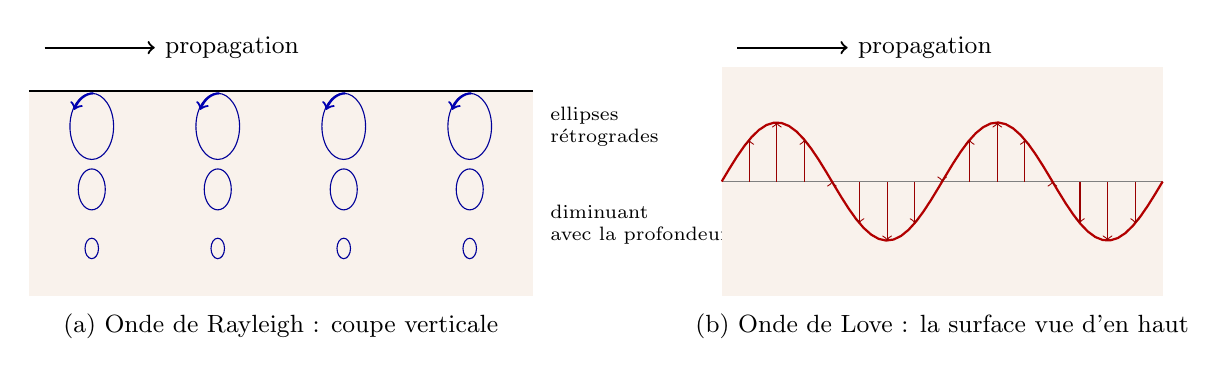
\begin{tikzpicture}[font=\small, x=1cm, y=1cm]
% Rayleigh: vertical section
\fill[brown!10] (0,0) rectangle (6.4,-2.6);
\draw[thick] (0,0) -- (6.4,0);
\draw[->, thick] (0.2,0.55) -- (1.6,0.55) node[right] {propagation};
\foreach \x/\s in {0.8/1, 2.4/-1, 4.0/1, 5.6/-1} {
  \foreach \z/\a in {-0.45/0.42, -1.25/0.26, -2.0/0.13} {
    \draw[blue!60!black] (\x,\z) ellipse ({0.66*\a} and {\a});
  }
}
\foreach \x in {0.8, 2.4, 4.0, 5.6} {
  \draw[->, blue!70!black, thick] (\x+0.02,-0.03) arc (90:150:{0.28} and {0.42});
}
\node[anchor=north] at (3.2,-2.7) {(a) Onde de Rayleigh~: coupe verticale};
\node[anchor=west, font=\scriptsize, align=left] at (6.5,-0.45) {ellipses\\ rétrogrades};
\node[anchor=west, font=\scriptsize, align=left] at (6.5,-1.7) {diminuant\\ avec la profondeur};
% Love: plan view of the surface
\begin{scope}[xshift=8.8cm]
\fill[brown!10] (0,0.3) rectangle (5.6,-2.6);
\draw[->, thick] (0.2,0.55) -- (1.6,0.55) node[right] {propagation};
\draw[gray, thin] (0,-1.15) -- (5.6,-1.15);
\draw[red!70!black, thick, domain=0:5.6, samples=60] plot (\x,{-1.15+0.75*sin(\x*360/2.8)});
\foreach \x in {0.35,0.7,...,5.3} {
  \pgfmathsetmacro{\d}{0.75*sin(\x*360/2.8)}
  \draw[->, red!60!black] (\x,-1.15) -- (\x,{-1.15+\d});
}
\node[anchor=north] at (2.8,-2.7) {(b) Onde de Love~: la surface vue d'en haut};
\end{scope}
\end{tikzpicture}

\par\smallskip{\small Mouvements des particules des deux ondes de surface (schéma).
(a) Une \omterm{def:b3:seismology-imaging:surface-waves}{onde de Rayleigh} déplace le sol dans le plan vertical de propagation,
selon des ellipses qui s'inversent vers le haut (rétrogrades) près de la surface et
diminuent avec la profondeur. (b) Une \omterm{def:b3:seismology-imaging:surface-waves}{onde de Love} déplace le sol horizontalement, perpendiculairement à la
direction de propagation~: les flèches montrent le déplacement à un instant donné
le long d'une ligne de la surface.}
\label{fig:b3:seismology-imaging:particle-motion}
\end{omfigure}

\begin{theorem}[Dispersion des ondes de Love dans une couche reposant sur un demi-espace]\label{thm:b3:seismology-imaging:love}
Une couche d'épaisseur $H$, de module de cisaillement $\mu_1$ et de vitesse S $\beta_1$ repose sur un
demi-espace de module de cisaillement $\mu_2$ et de vitesse S $\beta_2 > \beta_1$. Une
\omterm{def:b3:seismology-imaging:surface-waves}{onde de Love} de pulsation $\omega$ et de nombre d'onde $k$ se propage avec la
vitesse de phase $c = \omega/k$, $\beta_1 < c < \beta_2$, si et seulement si
\[
  \tan\!\left(kH q_1\right) = \frac{\mu_2 q_2}{\mu_1 q_1},
  \qquad q_1 = \sqrt{\frac{c^2}{\beta_1^2} - 1},\quad
  q_2 = \sqrt{1 - \frac{c^2}{\beta_2^2}} .
\]
Le mode fondamental est la racine telle que $0 < kHq_1 < \pi/2$~; les harmoniques ont
$kHq_1$ dans $(n\pi, n\pi + \pi/2)$.
\end{theorem}

\begin{proof}
Prenons $x$ dans le sens de la propagation, $y$ horizontal et perpendiculaire à celui-ci, et $z$ orienté vers le bas à partir de
la surface libre, et cherchons un déplacement
$u_y = f(z)\,e^{i(kx - \omega t)}$, les autres composantes étant nulles. Chaque couche
obéit à l'équation d'onde $\partial^2 u_y/\partial t^2 = \beta^2\nabla^2 u_y$, d'où
$f'' = -k^2\left(c^2/\beta^2 - 1\right) f$. Dans la couche, $c > \beta_1$, et
$f = A\cos(kq_1z) + B\sin(kq_1z)$. Dans le demi-espace, $c < \beta_2$, et la
solution qui reste bornée en profondeur est $f = C\,e^{-kq_2(z - H)}$.
La contrainte de cisaillement sur un plan horizontal vaut $\mu\,\partial u_y/\partial z$.
En surface libre, elle s'annule~: $f'(0) = 0$, donc $B = 0$. En $z = H$, le
déplacement et la contrainte sont continus~:
\[
  A\cos(kq_1H) = C, \qquad -\mu_1 A\,kq_1\sin(kq_1H) = -\mu_2\,kq_2\,C .
\]
En divisant la seconde équation par la première, on obtient le résultat. Comme le
second membre est positif, $kHq_1$ se situe dans un quart de période où la
tangente est positive~; le plus petit intervalle de ce type donne le mode fondamental.
\end{proof}

Pour une période donnée, l'équation est résolue en $c$ par dichotomie~; la vitesse de
groupe se déduit de $U = \mathrm d\omega/\mathrm dk$. Aux courtes périodes
($kH$ grand), la racine est proche de $c = \beta_1$~: l'onde reste confinée dans la couche. Aux
longues périodes ($kH \to 0$), il faut que $kHq_1 \to 0$ avec un second membre
également petit, ce qui force $c \to \beta_2$~: l'onde pénètre profondément dans le
demi-espace et se propage à sa vitesse. Entre les deux, la vitesse de phase croît
régulièrement avec la période.

\begin{definition}[Dispersion des ondes de surface]\label{def:b3:seismology-imaging:dispersion}
La \emph{dispersion des ondes de surface}\index{dispersion des ondes de surface} est la dépendance
des vitesses de phase et de groupe d'une \omterm{def:b3:seismology-imaging:surface-waves}{onde de Rayleigh} ou de Love à sa période. Dans
une Terre stratifiée, elle résulte du fait qu'une onde de plus grande période atteint des profondeurs plus grandes
(environ un tiers de longueur d'onde pour le mode fondamental) et moyenne
une roche plus rapide~; les courbes de dispersion $c(T)$ et $U(T)$ mesurées entre un séisme
et une station, ou entre deux stations, sont inversées pour la vitesse S en
fonction de la profondeur.
\end{definition}

\begin{omfigure}
\begin{tikzpicture}
\begin{axis}[omrecord, xmode=log, width=0.82\linewidth, height=0.5\linewidth,
  xmin=3, xmax=150, ymin=3.3, ymax=4.6, log basis x=10,
  xtick={3,5,10,20,50,100,150}, xticklabels={3,5,10,20,50,100,150},
  xlabel={période $T$ (\unit{s})}, ylabel={vitesse (\unit{km.s^{-1}})},
  legend style={at={(0.03,0.62)}, anchor=west}, legend cell align=left]
\addplot[blue!70!black, thick] table[x=period, y=c] {figdata/out/bachelor-3-love_dispersion-curve.dat};
\addlegendentry{vitesse de phase $c$}
\addplot[red!70!black, thick] table[x=period, y=U] {figdata/out/bachelor-3-love_dispersion-curve.dat};
\addlegendentry{vitesse de groupe $U$}
\draw[gray, dashed] (axis cs:3,3.5) -- (axis cs:150,3.5);
\draw[gray, dashed] (axis cs:3,4.5) -- (axis cs:150,4.5);
\node[font=\scriptsize, anchor=south] at (axis cs:80,3.5) {$\beta_1 = 3.5$};
\node[font=\scriptsize, anchor=south west] at (axis cs:3.1,4.5) {$\beta_2 = 4.5$};
\addplot[only marks, mark=*, mark size=1.4pt, red!70!black] coordinates {(19.2,3.384)};
\node[font=\scriptsize, anchor=south, red!70!black] at (axis cs:19.2,3.39) {phase d'Airy};
\end{axis}
\end{tikzpicture}

\par\smallskip{\small \omterm{def:b3:seismology-imaging:surface-waves}{Ondes de Love} fondamentales dans une couche de \qty{35}{km}
($\beta_1 = \qty{3.5}{km.s^{-1}}$, \qty{2.7}{g.cm^{-3}}) sur un demi-espace
($\beta_2 = \qty{4.5}{km.s^{-1}}$, \qty{3.3}{g.cm^{-3}}), modèle arrondi de croûte
continentale posée sur le manteau, calculé à partir du
\cref{thm:b3:seismology-imaging:love}. La vitesse de phase croît de la
vitesse S de la couche à celle du demi-espace~; la vitesse de groupe est plus faible et présente un
minimum, \qty{3.384}{km.s^{-1}} à \qty{19.2}{s}, où des ondes de périodes voisines
arrivent ensemble sous la forme d'une grande impulsion tardive (la phase d'Airy).}
\label{fig:b3:seismology-imaging:love}
\end{omfigure}

Sur ce modèle, la vitesse de phase à \qty{20}{s} vaut \qty{3.79}{km.s^{-1}} et à
\qty{100}{s} \qty{4.444}{km.s^{-1}}~; les vitesses de groupe valent 3.384 et
\qty{4.333}{km.s^{-1}}. Sur un sismogramme enregistré à quelques milliers de kilomètres
de distance, les longues périodes arrivent en premier et les ondes à \qty{20}{s} en dernier, de sorte que le
train d'ondes s'étire en une longue oscillation qui se raccourcit lentement. Mesurer
la vitesse de groupe à de nombreuses périodes, le long de nombreux trajets, donne des cartes
de l'épaisseur de la croûte et du manteau supérieur, indépendantes des temps
de trajet des ondes de volume.

\section{La Terre résonne~: modes propres}

Une onde de surface de très longue période a une longueur d'onde comparable
au rayon de la Terre~; elle fait le tour du globe et se recoupe elle-même. Les ondes qui
interfèrent de façon constructive sont les ondes stationnaires de la sphère entière, ses modes
propres, et après un grand séisme ce sont les derniers signaux à s'éteindre.
Leur théorie, un problème aux valeurs propres pour la Terre élastique et auto-gravitante,
dépasse le cadre de ce chapitre~; leur description, elle, ne le fait pas.

Les modes d'une Terre à symétrie sphérique forment deux familles. Dans les
modes \emph{toroïdaux}, ${}_nT_\ell$, le mouvement est horizontal, une torsion de
couches sphériques les unes par rapport aux autres, sans variation de rayon ni de volume~: les
ondes stationnaires des \omterm{def:b3:seismology-imaging:surface-waves}{ondes de Love}. Dans les modes \emph{sphéroïdaux}, ${}_nS_\ell$,
le mouvement a une composante radiale et une composante horizontale, et la Terre change de forme~: les
ondes stationnaires des \omterm{def:b3:seismology-imaging:surface-waves}{ondes de Rayleigh}, couplées aux ondes de volume et à la gravité.
L'indice $\ell$ est le degré angulaire, soit le nombre de lignes nodales du
motif à la surface~; $n$ compte les nœuds du mouvement en fonction du rayon, $n = 0$
pour le mode fondamental. Le mode sphéroïdal le plus grave, ${}_0S_2$, étire la
Terre alternativement en sphéroïde allongé puis aplati~; le mode toroïdal le plus grave
${}_0T_2$ tord les hémisphères nord et sud en sens opposés. Leurs
périodes observées sont~:
\begin{center}
\small
% ledger: seis5:modes-T, seis5:modes-S
\begin{tabular}{lcccc}
\hline
mode & ${}_0T_2$ & ${}_1T_2$ & ${}_0T_3$ & ${}_1T_3$ \\
période (\unit{min}) & 44.01 & 12.61 & 28.43 & 11.59 \\
\hline
mode & ${}_0S_2$ & ${}_1S_2$ & ${}_0S_3$ & ${}_1S_3$ \\
période (\unit{min}) & 53.89 & 24.51 & 35.56 & 17.68 \\
\hline
\end{tabular}
\end{center}
Chaque période est une moyenne sur toute la planète de ses modules élastiques et
de sa masse volumique, pondérée par les zones où le mode se déplace~: les modes toroïdaux
ne sont sensibles qu'au manteau solide et à la croûte, les modes sphéroïdaux aussi au noyau. Ajuster les
périodes de centaines de modes est la seule façon sismologique de peser
l'intérieur~: elle contraint la masse volumique, et pas seulement les vitesses, et PREM a été conçu pour
les ajuster ensemble aux temps de trajet. La rotation et l'ellipticité
de la Terre scindent chaque mode de degré $\ell$ en $2\ell + 1$
fréquences légèrement différentes, analogue de l'effet Zeeman.

\begin{history}[La Terre après le séisme chilien]
Le séisme chilien de 1960 fut enregistré par des sismomètres pendulaires à longue période
et par des extensomètres, instruments qui mesurent la variation de longueur
d'une longue tige ou d'un fil horizontal ancré dans la roche. L'analyse spectrale de quelques jours de
l'enregistrement a montré des pics nets aux périodes prévues des modes les plus graves~: la
Terre entière avait été mise en résonance, et les prévisions de la théorie élastique
d'une Terre sphérique et auto-gravitante furent vérifiées. L'enregistrement de l'extensomètre
d'Isabella, en Californie, fut analysé à nouveau en 1978 avec des méthodes plus modernes
méthodes~: il montra clairement le dédoublement de ${}_0T_3$, ${}_0T_4$, ${}_0S_4$
et ${}_0S_5$ dus à la rotation et à l'ellipticité de la Terre, et confirma que
celui de ${}_0S_2$ et ${}_0S_3$.
% ledger: stein78:chile-modes, usgs5:chile1960
La sismologie des modes propres, née d'un seul séisme, s'appuie aujourd'hui sur les réseaux
de stations à très large bande qui enregistrent chaque grand séisme.
\end{history}

\section{Problèmes inverses linéaires}\label{sec:b3:seismology-imaging:inverse}

Toutes les méthodes de ce chapitre jusqu'ici calculent des données à partir d'un modèle. La tâche de
l'imagerie est l'opération inverse.

\begin{definition}[Problème direct, problème inverse]\label{def:b3:seismology-imaging:inverse}
Soit un modèle de la Terre décrit par un vecteur $\mathbf m$ de $M$ paramètres
et les observations par un vecteur $\mathbf d$ de $N$ données. Le \emph{problème
direct}\index{problème direct} consiste à calculer les données $\mathbf d = g(\mathbf m)$
que produirait un modèle donné selon une théorie physique. Le \emph{problème
inverse}\index{problème inverse} consiste à estimer le modèle à partir de données entachées
d'erreurs, $\mathbf d = g(\mathbf m) + \mathbf e$, et à préciser avec quelle précision chaque partie
du modèle est déterminée. Le problème est linéaire lorsque $g(\mathbf m) =
\mathsf G\mathbf m$ pour une matrice $N\times M$ fixée $\mathsf G$, appelée noyau.
\end{definition}

Ajuster une droite à des temps de trajet est un \omterm{def:b3:seismology-imaging:inverse}{problème inverse} linéaire à
$M = 2$ paramètres (exercice~7)~; une tomographie en temps de trajet en comporte des
milliers. Trois cas se présentent. Si $N > M$ et que les données contraignent chaque
paramètre, le problème est \emph{surdéterminé}~: aucun modèle ne reproduit chaque
donnée exactement, et le meilleur est cherché au sens statistique. Si une combinaison de
paramètres laisse les données inchangées ($\mathsf G\mathbf m_0 = \mathbf 0$ pour
un $\mathbf m_0 \ne \mathbf 0$), le problème est \emph{sous-déterminé} dans cette
direction, et aucune quantité de données de ce type ne pourra la fixer. Les problèmes réels sont
mixtes~: surdéterminés dans certaines parties du modèle et sous-déterminés dans
d'autres.

\begin{theorem}[Estimation par moindres carrés pondérés]\label{thm:b3:seismology-imaging:wls}
Soit $\mathbf d = \mathsf G\mathbf m + \mathbf e$, où les erreurs $\mathbf e$
sont de moyenne nulle et la matrice de covariance $\mathsf C_d$ (diagonale
$\sigma_i^2$ pour des erreurs indépendantes). Si la matrice
$\mathsf N = \mathsf G^{\mathsf T}\mathsf C_d^{-1}\mathsf G$ est inversible, le
modèle qui minimise l'écart d'ajustement
\[
  \chi^2(\mathbf m) = (\mathbf d - \mathsf G\mathbf m)^{\mathsf T}\mathsf C_d^{-1}
  (\mathbf d - \mathsf G\mathbf m)
\]
est l'\emph{estimation par moindres carrés pondérés}\index{estimation par moindres carrés pondérés}
\[
  \hat{\mathbf m} = \mathsf N^{-1}\mathsf G^{\mathsf T}\mathsf C_d^{-1}\mathbf d ,
\]
elle est sans biais, et sa matrice de covariance est
$\mathsf C_{\hat m} = \mathsf N^{-1}$.
\end{theorem}

\begin{proof}
$\chi^2$ est une fonction quadratique de $\mathbf m$, de gradient
$-2\mathsf G^{\mathsf T}\mathsf C_d^{-1}(\mathbf d - \mathsf G\mathbf m)$, qui
s'annule pour les équations normales $\mathsf N\mathbf m = \mathsf G^{\mathsf T}
\mathsf C_d^{-1}\mathbf d$~; la matrice hessienne $2\mathsf N$ est définie positive lorsque
$\mathsf N$ est inversible (elle vaut alors $\mathbf x^{\mathsf T}\mathsf N\mathbf x =
\|\mathsf C_d^{-1/2}\mathsf G\mathbf x\|^2 > 0$ pour $\mathbf x \ne 0$), de sorte que le
point stationnaire est le minimum. Écrivons $\hat{\mathbf m} = \mathsf H\mathbf d$ avec
$\mathsf H = \mathsf N^{-1}\mathsf G^{\mathsf T}\mathsf C_d^{-1}$. Alors
$\mathsf H\mathsf G = \mathsf I$, donc $\hat{\mathbf m} = \mathbf m + \mathsf H\mathbf e$
a pour moyenne $\mathbf m$, et sa covariance vaut
$\mathsf H\mathsf C_d\mathsf H^{\mathsf T} =
\mathsf N^{-1}\mathsf G^{\mathsf T}\mathsf C_d^{-1}\mathsf C_d\mathsf C_d^{-1}
\mathsf G\mathsf N^{-1} = \mathsf N^{-1}$.
\end{proof}

Les pondérations font ce que l'intuition demande~: une donnée dont l'erreur est
deux fois plus faible compte quatre fois plus. La matrice de covariance donne à chaque paramètre son écart type
$\sqrt{(\mathsf N^{-1})_{jj}}$ et les corrélations entre paramètres. Si le modèle
est juste et les erreurs gaussiennes, le $\chi^2$ minimal suit une loi du $\chi^2$
à $N - M$ degrés de liberté~: une valeur très supérieure à $N - M$ signifie que les erreurs
ont été sous-estimées ou que le modèle est trop simple~; une valeur très inférieure, que les
erreurs ont été surestimées.

Lorsque $\mathsf N$ est singulière ou presque, l'estimation n'existe pas ou est
dominée par le bruit amplifié dans les directions mal contraintes. La solution
usuelle consiste à chercher un modèle qui ajuste raisonnablement les données et
qui n'est pas inutilement grand.

\begin{definition}[Moindres carrés amortis, courbe de compromis]\label{def:b3:seismology-imaging:damped}
Pour un paramètre d'amortissement $\varepsilon > 0$, l'estimation par \emph{moindres carrés
amortis}\index{moindres carrés amortis} est le modèle qui minimise
\[
  \Phi_\varepsilon(\mathbf m) = \chi^2(\mathbf m) + \varepsilon^2\|\mathbf m\|^2 ,
  \qquad
  \mathbf m_\varepsilon = \left(\mathsf N + \varepsilon^2\mathsf I\right)^{-1}
  \mathsf G^{\mathsf T}\mathsf C_d^{-1}\mathbf d .
\]
La \emph{courbe de compromis}\index{courbe de compromis} est la courbe décrite, lorsque
$\varepsilon$ varie, par le couple (taille du modèle $\|\mathbf m_\varepsilon\|$,
écart d'ajustement $\chi^2(\mathbf m_\varepsilon)$)~: un faible amortissement ajuste étroitement les données
avec un modèle grand et irrégulier, un fort amortissement donne un modèle petit et un ajustement médiocre.
\end{definition}

La formule se retrouve comme dans le \cref{thm:b3:seismology-imaging:wls}~: le gradient
de $\Phi_\varepsilon$ vaut $-2\mathsf G^{\mathsf T}\mathsf C_d^{-1}(\mathbf d -
\mathsf G\mathbf m) + 2\varepsilon^2\mathbf m$, et $\mathsf N + \varepsilon^2
\mathsf I$ est toujours inversible, puisque ses valeurs propres sont celles de
$\mathsf N$ (toutes $\ge 0$) augmentées de $\varepsilon^2$. L'amortissement se choisit en général
près du coude de la \omterm{def:b3:seismology-imaging:damped}{courbe de compromis}, ou de sorte que $\chi^2$ soit voisin du
nombre de données, c'est-à-dire l'écart d'ajustement attendu pour les seules erreurs. Le prix
à payer est que l'estimation n'est plus sans biais.

\begin{definition}[Matrice de résolution du modèle]\label{def:b3:seismology-imaging:resolution}
Pour une estimation linéaire $\mathbf m_\varepsilon = \mathsf H_\varepsilon \mathbf d$
du modèle $\mathbf m$ à partir des données $\mathbf d = \mathsf G\mathbf m + \mathbf e$,
la \emph{matrice de résolution du modèle}\index{matrice de résolution du modèle} est
$\mathsf R = \mathsf H_\varepsilon\mathsf G$, de sorte que
\[
  \mathbf m_\varepsilon = \mathsf R\,\mathbf m + \mathsf H_\varepsilon\mathbf e .
\]
Pour les \omterm{def:b3:seismology-imaging:damped}{moindres carrés amortis}, $\mathsf R = (\mathsf N + \varepsilon^2\mathsf I)^{-1}
\mathsf N$. La ligne $j$ de $\mathsf R$ montre comment l'estimation du paramètre $j$
moyenne les vrais paramètres~; $\mathsf R = \mathsf I$ signifie une résolution parfaite.
\end{definition}

{\sloppy Si $\mathsf N$ possède les vecteurs propres orthonormés $\mathbf u_k$ et les valeurs
propres $\lambda_k$, alors $\mathsf R = \sum_k \frac{\lambda_k}{\lambda_k + \varepsilon^2}
\mathbf u_k\mathbf u_k^{\mathsf T}$~: les directions que les données contraignent bien
($\lambda_k \gg \varepsilon^2$) passent presque inchangées, celles qu'elles contraignent
mal sont atténuées. La trace de $\mathsf R$ compte les paramètres que les données
résolvent effectivement, et la covariance de l'estimation,
$\mathsf H_\varepsilon\mathsf C_d\mathsf H_\varepsilon^{\mathsf T}$, diminue à mesure
que la résolution augmente~: l'amortissement échange la résolution contre la stabilité.\par}

\begin{omfigure}
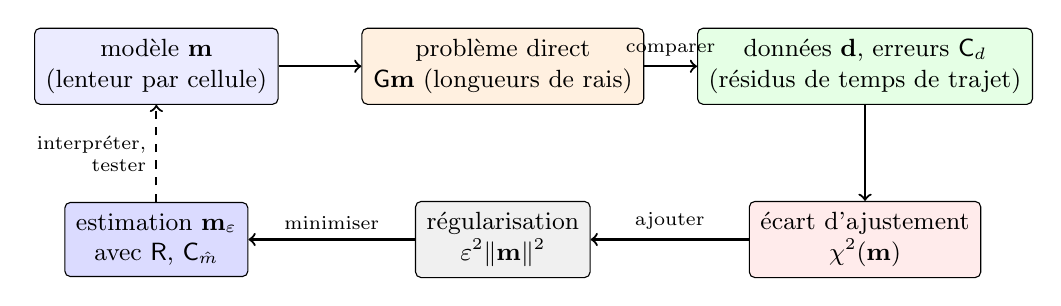
\begin{tikzpicture}[font=\small, node distance=0.5cm,
  box/.style={draw, rounded corners=2pt, fill=#1, minimum height=0.9cm, align=center, inner sep=4pt},
  box/.default=gray!8]
\node[box=blue!8] (m) at (0,0) {modèle $\mathbf m$\\(lenteur par cellule)};
\node[box=orange!12] (g) at (4.4,0) {problème direct\\$\mathsf G\mathbf m$ (longueurs de rais)};
\node[box=green!10] (d) at (9.0,0) {données $\mathbf d$, erreurs $\mathsf C_d$\\(résidus de temps de trajet)};
\node[box=red!8] (mis) at (9.0,-2.2) {écart d'ajustement\\$\chi^2(\mathbf m)$};
\node[box=gray!12] (reg) at (4.4,-2.2) {régularisation\\$\varepsilon^2\|\mathbf m\|^2$};
\node[box=blue!14] (est) at (0,-2.2) {estimation $\mathbf m_\varepsilon$\\avec $\mathsf R$, $\mathsf C_{\hat m}$};
\draw[->, thick] (m) -- (g);
\draw[->, thick] (g) -- node[above, font=\scriptsize] {comparer} (d);
\draw[->, thick] (d) -- (mis);
\draw[->, thick] (mis) -- node[above, font=\scriptsize] {ajouter} (reg);
\draw[->, thick] (reg) -- node[above, font=\scriptsize] {minimiser} (est);
\draw[->, thick, dashed] (est) -- node[left, font=\scriptsize, align=right] {interpréter,\\tester} (m);
\end{tikzpicture}

\par\smallskip{\small La boucle du \omterm{def:b3:seismology-imaging:inverse}{problème inverse} linéaire (schéma). Le
\omterm{def:b3:seismology-imaging:inverse}{problème direct} prédit des données à partir d'un modèle~; l'écart d'ajustement, pondéré par les
erreurs sur les données, mesure le désaccord~; le terme de régularisation maintient le modèle
petit~; minimiser leur somme donne l'estimation, qui ne s'interprète qu'avec
sa matrice de résolution et sa covariance.}
\label{fig:b3:seismology-imaging:inverse-loop}
\end{omfigure}

\section{Tomographie sismique}\label{sec:b3:seismology-imaging:tomography}

\begin{definition}[Tomographie sismique, résidu de temps de trajet]\label{def:b3:seismology-imaging:tomography}
Le \emph{résidu de temps de trajet}\index{résidu de temps de trajet} d'une arrivée est le
temps de trajet observé moins le temps prédit par un modèle de référence,
$\delta t = T_{\text{obs}} - T_{\text{ref}}$, après correction de la localisation
de la source et de son instant d'origine, de l'altitude de la station et de
l'aplatissement de la Terre. La \emph{tomographie sismique}\index{tomographie sismique} est
l'estimation des écarts tridimensionnels des vitesses sismiques par rapport à un
modèle de référence, $\delta v(\mathbf x)$, à partir d'un grand ensemble de résidus
(ou de sismogrammes complets), en résolvant un \omterm{def:b3:seismology-imaging:inverse}{problème inverse}.
\end{definition}

On note $s = 1/v$ la lenteur. Le temps de trajet le long d'un rai $\Gamma$ est
$T = \int_\Gamma s\,\mathrm dl$~; mais le rai lui-même dépend des vitesses,
ce qui semble rendre le problème non linéaire. La réponse au premier ordre est que
cela n'a pas d'importance.

\begin{proposition}[Résidu de temps de trajet linéarisé]\label{prop:b3:seismology-imaging:linear}
Si la lenteur du modèle de référence $s_0$ est perturbée en $s_0 + \delta s$,
le temps de trajet entre deux points fixes varie, au premier ordre en
$\delta s$, de
\[
  \delta t = \int_{\Gamma_0}\delta s\,\mathrm dl ,
\]
l'intégrale étant prise le long du rai $\Gamma_0$ du modèle de référence~; l'anomalie
relative de vitesse vaut $\delta v/v_0 = -\delta s/s_0$ au même ordre.
\end{proposition}

\begin{proof}
D'après le principe de Fermat, le rai $\Gamma_0$ rend le temps de trajet
$\int s_0\,\mathrm dl$ stationnaire parmi les trajets voisins~: déplacer le trajet
d'une petite quantité $\epsilon$ ne modifie le temps que d'un terme d'ordre $\epsilon^2$.
Le nouveau rai $\Gamma$ diffère de $\Gamma_0$ d'une quantité d'ordre $\delta s$~;
donc $\int_\Gamma(s_0 + \delta s)\,\mathrm dl = \int_{\Gamma_0}s_0\,\mathrm dl +
O(\delta s^2) + \int_{\Gamma_0}\delta s\,\mathrm dl + O(\delta s^2)$. Enfin
$\delta(1/s) = -\delta s/s_0^2$, donc $\delta v/v_0 = -\delta s/s_0$.
\end{proof}

Découper la région en $M$ cellules de perturbation de lenteur uniforme $\delta s_j$.
Le résidu du rai $i$ devient $\delta t_i = \sum_j L_{ij}\,\delta s_j$, où
$L_{ij}$ est la longueur du rai de référence $i$ dans la cellule $j$~: il s'agit d'un
\omterm{def:b3:seismology-imaging:inverse}{problème inverse} linéaire dont le noyau est la matrice des longueurs de rais, dont presque
tous les coefficients sont nuls. Les résidus sont faibles~: dans un manteau à
\qty{8}{km.s^{-1}}, une région large de \qty{200}{km} et plus rapide de
\qty{3}{\percent} avance un rai vertical d'environ \qty{0.7}{s} (exercice 9).

\begin{method}[Une tomographie par temps de trajet]\label{met:b3:seismology-imaging:tomo}
\begin{enumerate}
  \item Pointer les temps d'arrivée d'une phase (disons P) à toutes les stations, pour
        des séismes dont la localisation est bien connue~; calculer les résidus
        par rapport à une \omterm{def:b3:seismology-imaging:tables}{table de temps de trajet}, corrigés de l'aplatissement et de
        l'altitude de la station.
  \item Tracer les rais de référence et découper la région en cellules (ou développer
        $\delta s$ sur des fonctions lisses)~; remplir la matrice des longueurs de rais.
  \item Affecter à chaque résidu son erreur, déduite de la précision du pointé, et résoudre
        le problème des \omterm{def:b3:seismology-imaging:damped}{moindres carrés amortis} pour une gamme de valeurs d'amortissement~;
        tracer la \omterm{def:b3:seismology-imaging:damped}{courbe de compromis} et choisir l'amortissement près de son coude.
  \item Tester la résolution~: calculer les résidus qu'un modèle synthétique connu
        donnerait par les mêmes rais, ajouter du bruit, les inverser avec le même
        amortissement, et comparer.
  \item N'interpréter que les anomalies que le test montre que les rais peuvent
        restituer, leurs amplitudes étant considérées comme des bornes inférieures.
\end{enumerate}
\end{method}

\begin{definition}[Test en damier]\label{def:b3:seismology-imaging:checkerboard}
Un \emph{test en damier}\index{test en damier} est un test de résolution dans
lequel le modèle synthétique est un motif régulier de cellules alternativement rapides
et lentes~: des résidus synthétiques calculés par la géométrie réelle des rais, avec un bruit
de l'ordre des erreurs réelles, sont inversés avec la même paramétrisation et le même
amortissement. Là où le motif est retrouvé, des structures de cette taille peuvent être
résolues~; là où il est estompé ou perdu, elles ne le peuvent pas.
\end{definition}

Les figures ci-dessous réalisent le test sur une coupe de modèle large de
\qty{800}{km} et profonde de \qty{400}{km}, découpée en 128 cellules de \qty{50}{km}. Vingt
sources se trouvent le long de sa base et trente-deux stations le long de son sommet, et seuls
les rais situés à moins de \ang{45} de la verticale sont utilisés~: 480 rais qui remontent tous
fortement, la géométrie des rais de séismes lointains remontant sous un réseau. Le modèle
synthétique comporte des blocs de $2\times2$ cellules, \qty{3}{\percent} plus rapides ou
plus lents autour de \qty{8}{km.s^{-1}}~; les résidus portent un bruit gaussien de
\qty{0.05}{s}.
% figdata: tomo_checkerboard.py (invented geometry; no real data)

\begin{omfigure}
\begin{tikzpicture}
\begin{groupplot}[group style={group size=2 by 2, horizontal sep=0.9cm, vertical sep=1.25cm},
  width=0.46\linewidth, height=0.3\linewidth, xmin=0, xmax=800, ymin=0, ymax=400,
  axis on top, enlargelimits=false, tick label style={font=\scriptsize},
  title style={font=\small, yshift=-1ex},
  colormap={tomo}{rgb255(0cm)=(178,24,43); rgb255(1cm)=(244,165,130); rgb255(2cm)=(247,247,247); rgb255(3cm)=(146,197,222); rgb255(4cm)=(33,102,172)},
  point meta min=-4, point meta max=4]
\nextgroupplot[title={(a) modèle synthétique}, ylabel={\scriptsize hauteur (km)}]
\addplot[matrix plot*, mesh/cols=16, point meta=explicit] table[x=x, y=y, meta=dv] {figdata/out/bachelor-3-tomo_checkerboard-true.dat};
\nextgroupplot[title={(b) un échantillon des 480 rais}, colormap/blackwhite]
\addplot[gray!70!black, thin, unbounded coords=jump] table[x=x, y=y] {figdata/out/bachelor-3-tomo_checkerboard-rays.dat};
\addplot[only marks, mark=triangle*, mark size=1.6pt, black, clip=false] table[x=x, y=y] {figdata/out/bachelor-3-tomo_checkerboard-receivers.dat};
\addplot[only marks, mark=star, mark size=1.8pt, red!70!black, clip=false] table[x=x, y=y] {figdata/out/bachelor-3-tomo_checkerboard-sources.dat};
\nextgroupplot[title={(c) retrouvé, $\varepsilon = \qty{3}{km}$}, ylabel={\scriptsize hauteur (km)}, xlabel={\scriptsize distance (km)}]
\addplot[matrix plot*, mesh/cols=16, point meta=explicit] table[x=x, y=y, meta=dv] {figdata/out/bachelor-3-tomo_checkerboard-rec-low.dat};
\nextgroupplot[title={(d) retrouvé, $\varepsilon = \qty{60}{km}$}, xlabel={\scriptsize distance (km)},
  colorbar right, colorbar style={width=0.2cm, ytick={-4,-2,0,2,4}, ylabel={\scriptsize $\delta v/v$ (\%)}, tick label style={font=\scriptsize}}]
\addplot[matrix plot*, mesh/cols=16, point meta=explicit] table[x=x, y=y, meta=dv] {figdata/out/bachelor-3-tomo_checkerboard-rec-high.dat};
\end{groupplot}
\end{tikzpicture}

\par\smallskip{\small Un \omterm{def:b3:seismology-imaging:checkerboard}{test en damier} (géométrie fictive). (a) Le
modèle synthétique~: blocs de \qty{100}{km} de côté, \qty{3}{\percent} plus rapides (bleu) ou
plus lents (rouge). (b) Les 20 sources (étoiles), les 32
stations (triangles) et quelques rais, tous à moins de \ang{45} de la verticale. (c) Avec un
faible amortissement, les blocs sont retrouvés, mais bruités, avec des anomalies allant jusqu'à
environ \qty{8}{\percent} là où peu de rais se croisent (les couleurs saturent à
\qty{4}{\percent}). (d) Avec un fort amortissement, le motif est net, mais son
amplitude est réduite, surtout le long des bords latéraux, où peu de rais se croisent
et tous sous des angles semblables.}
\label{fig:b3:seismology-imaging:checkerboard}
\end{omfigure}

\begin{omfigure}
\begin{tikzpicture}
\begin{axis}[omrecord, width=0.62\linewidth, height=0.42\linewidth,
  xlabel={norme du modèle $\|\delta v/v\|$ (\unit{\percent})},
  ylabel={écart d'ajustement $\|\mathsf G\mathbf m - \mathbf d\|$ (\unit{s})}, xmin=0, xmax=42, ymin=0, ymax=12]
\addplot[blue!70!black, thick] table[x=norm, y=misfit] {figdata/out/bachelor-3-tomo_checkerboard-tradeoff.dat};
\addplot[only marks, mark=*, mark size=1.8pt, red!70!black] coordinates {(38.84,0.862) (29.42,1.159)};
\node[font=\scriptsize, anchor=south, red!70!black] at (axis cs:38.84,1.3) {$\varepsilon = 3$};
\node[font=\scriptsize, anchor=east, red!70!black] at (axis cs:28.6,0.55) {$\varepsilon = 60$};
\draw[gray, dashed] (axis cs:0,1.095) -- (axis cs:42,1.095);
\node[font=\scriptsize, anchor=south west] at (axis cs:1,1.15) {attendu d'après le bruit};
\draw[green!45!black, densely dotted] (axis cs:33.94,0) -- (axis cs:33.94,12);
\node[font=\scriptsize, anchor=north west, green!45!black] at (axis cs:34.2,11.8) {modèle vrai};
\node[font=\scriptsize, anchor=west] at (axis cs:14,10.5) {fort amortissement};
\node[font=\scriptsize, anchor=east] at (axis cs:41,3.2) {faible amortissement};
\end{axis}
\end{tikzpicture}

\par\smallskip{\small La \omterm{def:b3:seismology-imaging:damped}{courbe de compromis} du \omterm{def:b3:seismology-imaging:checkerboard}{test en damier}, pour des valeurs d'amortissement
$\varepsilon$ de 0.1 à \qty{1000}{km} (le noyau est exprimé en kilomètres,
avec des erreurs égales). Sur la partie plane, un amortissement supplémentaire ne coûte presque rien en ajustement~:
le modèle se contracte en perdant du bruit. Le coude se situe là où l'écart d'ajustement dépasse le
niveau attendu du seul bruit, $\sigma\sqrt{480} = \qty{1.095}{s}$ ; les
deux modèles amortis de la figure précédente se trouvent de part et d'autre de ce coude,
et la norme du damier vrai, \qty{33.9}{\percent}, entre les deux. Au-delà du
coude, l'amortissement supprime des structures que les données exigent.}
\label{fig:b3:seismology-imaging:tradeoff}
\end{omfigure}

Le test illustre les trois limites de toute image tomographique. La résolution
est fixée par les rais~: là où tous les rais sont parallèles, une anomalie est étalée
le long de ceux-ci, et une cellule traversée par peu de rais est à peine contrainte. L'amortissement abaisse les
amplitudes~: les anomalies retrouvées sont des bornes inférieures.
Par ailleurs, l'image dépend du modèle de référence et du paramétrage~: seuls les
écarts au modèle de référence sont cartographiés, et rien de plus petit qu'une cellule n'est visible.
Sous ces réserves, les images globales des ondes P et S montrent les panneaux plongeants
du volume de première année (dans son chapitre sur la subduction) comme des régions rapides et tabulaires qui descendent
depuis les fosses, certaines s'aplatissant au-dessus de la discontinuité à 670~km, d'autres
plongeant dans le manteau inférieur~; et de larges régions lentes sous le Pacifique et
l'Afrique, au-dessus du noyau, avec des conduits lents plus étroits sous certains points chauds,
candidats aux panaches mantelliques du même volume.

\begin{inthefield}[Une station à large bande et un déploiement en fond océanique]
\begin{minipage}[t]{0.55\linewidth}\vspace{0pt}
Une station permanente à large bande est un lieu calme~: le sismomètre repose sur un
pilier en béton scellé au substratum rocheux, dans une chambre enterrée ou un court
tunnel, sous un écran thermique, car un courant d'air ou une variation de quelques centièmes de degré
incline l'instrument davantage qu'un séisme lointain. Ses trois composantes,
verticale, nord et est, sont numérisées en continu et envoyées à un centre de données
muni d'un horodatage par satellite. Pour imager une région située sous l'océan, une équipe
de terrain largue plutôt depuis un navire des sismomètres de fond océanique~: chacun coule sur une ancre,
enregistre pendant un an sur le fond marin, puis remonte à la surface lorsque le navire
revient et envoie un signal acoustique qui le libère. L'équipe lit alors
la dérive de son horloge, corrige les enregistrements et ajoute des milliers d'arrivées à la
tomographie.
\end{minipage}\hfill
\begin{minipage}[t]{0.42\linewidth}\vspace{0pt}
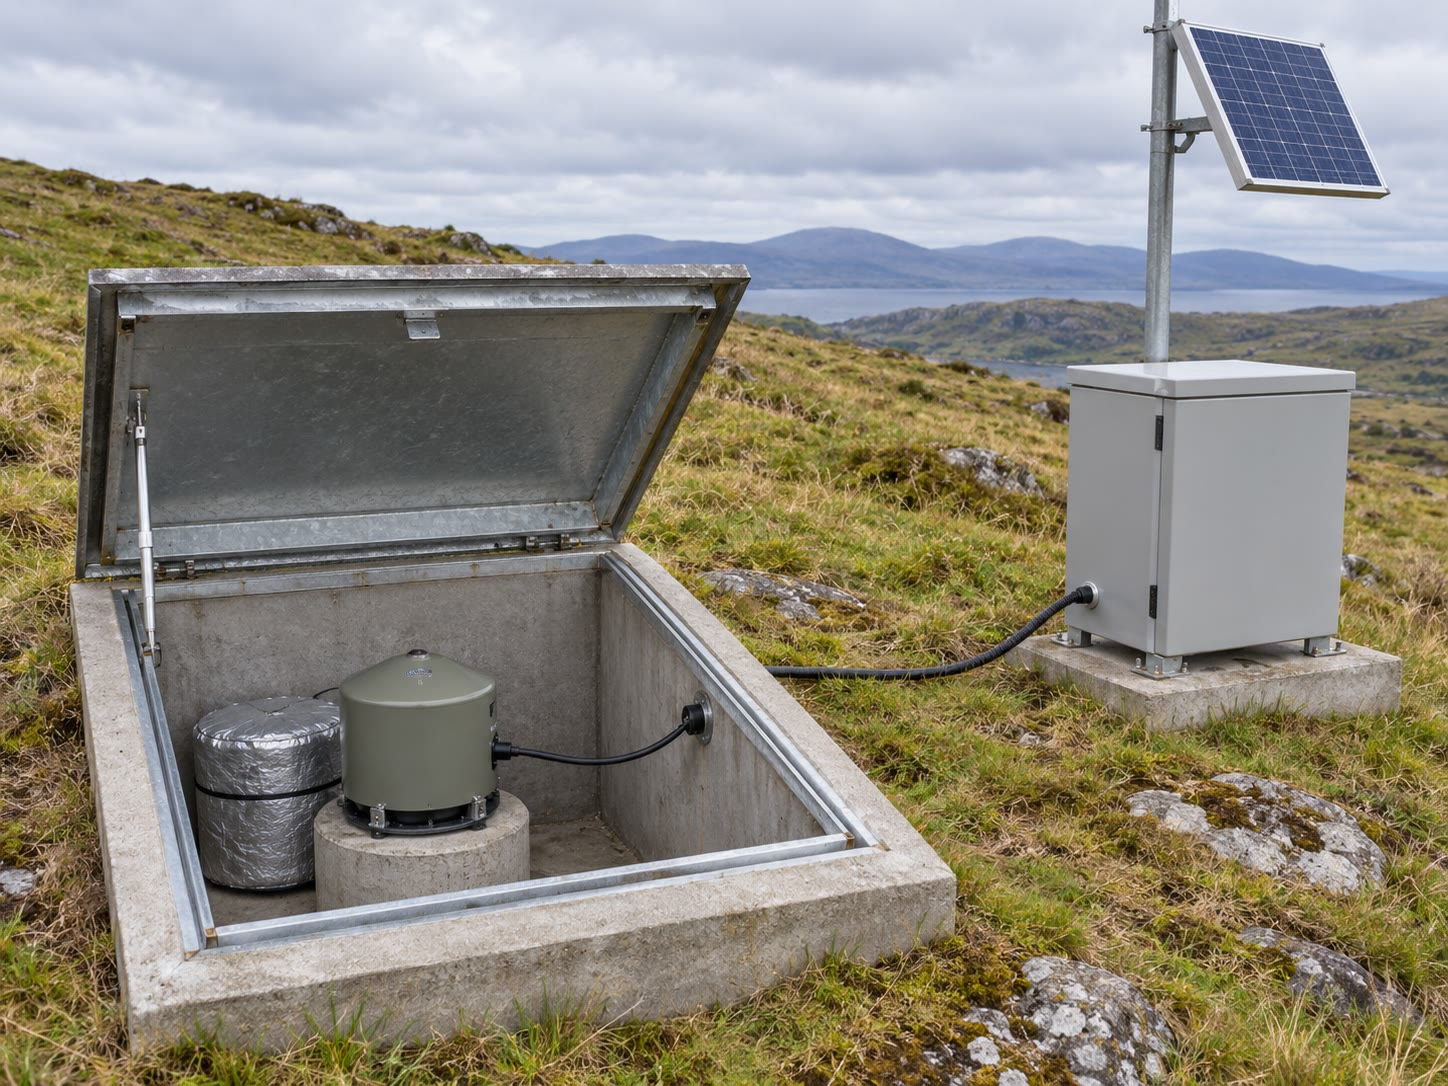
\includegraphics[width=\linewidth]{images/book5/ai/b3-seismic-vault.jpg}

{\scriptsize Un sismomètre à large bande sur son pilier, dans la chambre d'une station
(illustration générée par IA).}
\end{minipage}
\end{inthefield}

\section{Exercices}

\begin{exercise}[$\star$]\label{exo:b3:seismology-imaging:1}
Un rai P quitte la surface ($R = \qty{6371}{km}$, $v_0 = \qty{5.80}{km.s^{-1}}$)
avec le \omterm{def:b3:seismology-imaging:ray-parameter}{paramètre de rai} $p = \qty{500}{s.rad^{-1}}$. (a) Calculer son angle de départ.
(b) PREM donne des vitesses P de \qty{11.066}{km.s^{-1}} à \qty{771}{km} de profondeur
et \qty{11.245}{km.s^{-1}} à \qty{871}{km}. Calculer $r/v$ aux deux profondeurs et
déterminer la profondeur de retournement du rai par interpolation linéaire.
% ledger: ak135:crust, data:prem
\end{exercise}

\begin{exercise}[$\star$]\label{exo:b3:seismology-imaging:2}
Les temps P calculés avec PREM dans ce chapitre sont \qty{369.6}{s} à \ang{30}
et \qty{455.5}{s} à \ang{40}. (a) Estimer la pente de la courbe de temps de trajet
entre ces deux points, en \unit{s} par degré et en \unit{s.rad^{-1}}. (b) En déduire
la vitesse apparente du front d'onde le long de la surface, en
\unit{km.s^{-1}}. (c) Quelle est la vitesse P au \omterm{def:b3:seismology-imaging:ray-parameter}{point de retournement} du rai
arrivant à \ang{35}, s'il retourne au rayon \qty{5450}{km}~?
\end{exercise}

\begin{exercise}[$\star$]\label{exo:b3:seismology-imaging:3}
Dans le modèle d'\omterm{def:b3:seismology-imaging:surface-waves}{onde de Love} de ce chapitre, la couche a $\beta_1 =
\qty{3.5}{km.s^{-1}}$, $\rho_1 = \qty{2700}{kg.m^{-3}}$ et le demi-espace
$\beta_2 = \qty{4.5}{km.s^{-1}}$, $\rho_2 = \qty{3300}{kg.m^{-3}}$.
(a) Calculer les deux modules de cisaillement. (b) À \qty{20}{s}, la vitesse de phase vaut
\qty{3.79}{km.s^{-1}}~: calculer la longueur d'onde et la comparer à l'épaisseur de la couche,
\qty{35}{km}. (c) Avec des vitesses de groupe de \qty{3.384}{km.s^{-1}} à
\qty{20}{s} et \qty{4.333}{km.s^{-1}} à \qty{100}{s}, de combien de minutes les
ondes de 20~s arrivent-elles après celles de 100~s à une station située à \qty{4000}{km}~?
\end{exercise}

\begin{exercise}[$\star$]\label{exo:b3:seismology-imaging:4}
Les périodes observées de ${}_0S_2$ et ${}_0T_2$ sont \qty{53.89}{min} et
\qty{44.01}{min}. (a) Calculer leurs fréquences en \unit{mHz}. (b) Combien d'oscillations
chacun de ces modes accomplit-il en un jour~? (c) Deux pics spectraux ne peuvent être
séparés que si l'enregistrement dure au moins l'inverse de leur écart de fréquence.
Quelle doit être la durée d'un enregistrement pour séparer ces deux modes~?
% ledger: seis5:modes-S, seis5:modes-T
\end{exercise}

\begin{exercise}[$\star\star$]\label{exo:b3:seismology-imaging:5}
Dans une sphère de rayon $R$ et de vitesse uniforme $v$, les rais sont des cordes droites.
(a) Montrer que le rai atteignant $\Delta$ a pour temps de trajet
$T = 2R\sin(\Delta/2)/v$. (b) Avec $R = \qty{6371}{km}$ et
$v = \qty{10.0}{km.s^{-1}}$, calculer $T$ à \ang{30} et \ang{90}, et comparer
avec les temps PREM, \qty{369.6}{s} et \qty{779.7}{s}. (c) Expliquer pourquoi la
sphère uniforme est trop rapide à \ang{30} et trop lente à \ang{90}.
\end{exercise}

\begin{exercise}[$\star\star$]\label{exo:b3:seismology-imaging:6}
Sur un solide de Poisson ($\lambda = \mu$, donc $\alpha^2 = 3\beta^2$), la vitesse $c$
de l'\omterm{def:b3:seismology-imaging:surface-waves}{onde de Rayleigh} vérifie, avec $\xi = c^2/\beta^2$,
$(2 - \xi)^2 = 4\sqrt{1 - \xi/3}\,\sqrt{1 - \xi}$. (a) Élever au carré et montrer
que les racines vérifient $(\xi - 4)(3\xi^2 - 12\xi + 8) = 0$. (b) Montrer que la
seule racine avec $0 < \xi < 1$ est $\xi = 2 - 2/\sqrt3$, puis calculer $c/\beta$.
(c) Dans la croûte supérieure d'ak135, $\beta = \qty{3.46}{km.s^{-1}}$ : calculer la
vitesse de Rayleigh et le retard de l'\omterm{def:b3:seismology-imaging:surface-waves}{onde de Rayleigh} sur l'onde S à
\qty{1000}{km}.
% ledger: ak135:crust
\end{exercise}

\begin{exercise}[$\star\star$]\label{exo:b3:seismology-imaging:7}
Des arrivées d'ondes coniques à quatre stations d'une ligne de sismique réfraction, à 50, 100, 150 et
\qty{200}{km} du tir, sont de 9.0, 15.3, 21.5 et \qty{27.9}{s}, avec
des erreurs de 0.1, 0.1, 0.2 et \qty{0.2}{s}. Ajuster $T = a + bx$ par moindres carrés pondérés~:
écrire $\mathsf G$ et $\mathsf C_d$, former les équations normales, et
donner $a$, $b$, leurs erreurs-types, la vitesse $1/b$ avec son erreur, et le
$\chi^2$ minimal. L'ajustement est-il acceptable~?
\end{exercise}

\begin{exercise}[$\star\star$]\label{exo:b3:seismology-imaging:8}
Un rai traverse deux cellules, de longueurs \qty{30}{km} et \qty{40}{km}, et présente
un résidu de \qty{0.50}{s}. (a) Pourquoi $\mathsf N = \mathsf G^{\mathsf T}
\mathsf G$ est-elle singulière~? (b) Parmi les modèles qui ajustent exactement le résidu, celui
de plus petite norme est $\mathbf m = \mathsf G^{\mathsf T}(\mathsf G\mathsf
G^{\mathsf T})^{-1}\mathbf d$~: le calculer. (c) Calculer la matrice
$\mathsf R = \mathsf G^{\mathsf T}(\mathsf G\mathsf G^{\mathsf T})^{-1}\mathsf G$
et sa trace. (d) Si l'anomalie vraie vaut \qty{0.01}{s.km^{-1}} dans la première
cellule seulement, que retrouve-t-on~?
\end{exercise}

\begin{exercise}[$\star\star$]\label{exo:b3:seismology-imaging:9}
Une région du manteau en forme de panneau plongeant est \qty{3}{\percent} plus rapide que son environnement,
où $v = \qty{9.0}{km.s^{-1}}$. (a) Calculer le résidu d'un rai qui traverse
verticalement \qty{200}{km} de celle-ci, par la \cref{prop:b3:seismology-imaging:linear},
et de manière exacte. (b) Même question pour un rai traversant une épaisseur de \qty{100}{km} de celle-ci à
\ang{40} de la normale au panneau. (c) Quelle est l'erreur relative de la
linéarisation~?
\end{exercise}

\begin{exercise}[$\star\star\star$]\label{exo:b3:seismology-imaging:10}
Dans le \cref{thm:b3:seismology-imaging:love}, un harmonique d'ordre $n$ n'existe que
pour des périodes suffisamment courtes. (a) Montrer qu'à sa fréquence de coupure sa vitesse de phase vaut
$\beta_2$ et $kHq_1 = n\pi$. (b) En déduire la pulsation de coupure
$\omega_n = n\pi\beta_1\beta_2/\bigl(H\sqrt{\beta_2^2 - \beta_1^2}\bigr)$.
(c) Calculer la période de coupure du premier harmonique pour le modèle du chapitre
($H = \qty{35}{km}$, $\beta_1 = 3.5$, $\beta_2 = \qty{4.5}{km.s^{-1}}$).
(d) Montrer que le mode fondamental n'a pas de coupure, et que sa vitesse de phase
tend vers $\beta_1$ aux courtes périodes.
\end{exercise}

\begin{exercise}[$\star\star\star$]\label{exo:b3:seismology-imaging:11}
Reprendre le rai de l'exercice 8, avec une erreur de donnée unitaire. (a) Montrer que, pour tout
$\varepsilon > 0$, $(\mathsf G^{\mathsf T}\mathsf G + \varepsilon^2\mathsf
I)^{-1}\mathsf G^{\mathsf T} = \mathsf G^{\mathsf T}(\mathsf G\mathsf
G^{\mathsf T} + \varepsilon^2\mathsf I)^{-1}$. (b) En déduire la résolution amortie
matrice de résolution amortie $\mathsf R_\varepsilon = \mathsf G^{\mathsf T}\mathsf G/(\|\mathbf g\|^2 +
\varepsilon^2)$, où $\mathbf g = (30, 40)$, et sa trace. (c) Calculer la
trace et le résidu de données pour $\varepsilon^2 = 0$, 2500 et \num{10000}
(en \unit{km^2}). Décrire le compromis.
\end{exercise}

\begin{exercise}[$\star\star\star$]\label{exo:b3:seismology-imaging:12}
Dans la sphère uniforme de l'exercice 5~: (a) montrer par le
\cref{thm:b3:seismology-imaging:benndorf} que $p(\Delta) = (R/v)\cos(\Delta/2)$,
et le vérifier par la définition de $p$ (l'angle de départ d'une corde).
(b) Montrer que le rai atteignant $\Delta_1$ a son \omterm{def:b3:seismology-imaging:ray-parameter}{point de retournement} en $r_1 = R\cos(\Delta_1/2)$.
(c) En admettant que $\int_0^{\Delta_1}\operatorname{arccosh}\bigl(\cos(\Delta/2)
/\cos(\Delta_1/2)\bigr)\,\mathrm d\Delta = \pi\ln\bigl(1/\cos(\Delta_1/2)\bigr)$,
montrer que la formule de Herglotz--Wiechert restitue $r_1$ et la vitesse $v$.
\end{exercise}

\section{Problème~: le panneau sous la station K}

\begin{problem}[{Problème du week-end --- rais, ondes de Love et petite tomographie
sous une station fictive}]
\label{pb:b3:seismology-imaging:1}
% values: calc/ch01.py (invented station and models; Love-wave model as in the chapter)
La station K se trouve sur un continent au-dessus d'une zone de subduction. Ce problème exploite ses
enregistrements de trois façons~: des rais dans sa croûte, la dispersion des \omterm{def:b3:seismology-imaging:surface-waves}{ondes de Love} à travers elle,
et une petite tomographie du manteau sous-jacent.

\medskip
\noindent\textbf{Partie I --- Rais dans un gradient.} Sur des distances assez courtes pour
négliger la courbure de la Terre, la vitesse P sous K croît linéairement avec la profondeur,
$v(z) = v_0 + gz$, avec $v_0 = \qty{5.0}{km.s^{-1}}$ et
$g = \qty{0.05}{s^{-1}}$ ($z$ en km).
\begin{enumerate}
  \item Dans des couches planes, la loi de Snell conserve $p = \sin i/v$ constant. Un rai quitte
        K avec $\sin i_0 = 0.8$~: calculer $i_0$ et $p$.
  \item À quelle profondeur ce rai atteint-il son \omterm{def:b3:seismology-imaging:ray-parameter}{point de retournement}, et quelle est la vitesse à cet endroit~?
       \item Montrer que $\mathrm di/\mathrm ds = pg$ le long du rai, de sorte que c'est un
        arc de cercle~; donner son rayon et la profondeur de son centre.
  \item Calculer la distance horizontale $X$ à laquelle le rai revient à la
        surface.
  \item Montrer que $\mathrm dT = \mathrm di/(g\sin i)$ et calculer exactement le temps de
        trajet $T$.
  \item Calculer $X$ et $T$ pour $p = \qty{0.15}{s.km^{-1}}$, et vérifier que
        $\Delta T/\Delta X$ entre les deux rais se situe entre les deux valeurs
        de $p$.
\end{enumerate}

\noindent\textbf{Partie II --- Ondes de Love et croûte.} La croûte sous K est une
couche de vitesse S $\beta_1 = \qty{3.5}{km.s^{-1}}$ et de masse volumique
$\rho_1 = \qty{2.7}{g.cm^{-3}}$ reposant sur un manteau de $\beta_2 =
\qty{4.5}{km.s^{-1}}$, $\rho_2 = \qty{3.3}{g.cm^{-3}}$~; son épaisseur $H$ est
inconnue. Entre K et une station voisine, la vitesse de phase des \omterm{def:b3:seismology-imaging:surface-waves}{ondes de Love} est
mesurée~: \qty{3.99}{km.s^{-1}} à \qty{25}{s} et \qty{4.25}{km.s^{-1}} à
\qty{40}{s}.
\begin{enumerate}[resume]
  \item Calculer $\mu_1$ et $\mu_2$ en \unit{GPa}.
  \item À \qty{25}{s}, calculer $k$, $q_1$ et $q_2$.
  \item Résoudre l'équation de dispersion du mode fondamental pour $H$.
  \item Faire de même à \qty{40}{s}. Les deux résultats sont-ils cohérents~?
       \item Estimer la vitesse de groupe entre les deux périodes par
        $\Delta\omega/\Delta k$, et la comparer aux vitesses de phase.
  \item Calculer la longueur d'onde à chaque période, et expliquer pourquoi les deux
        périodes sondent la croûte et le manteau supérieur dans des
        proportions différentes.
\end{enumerate}

\noindent\textbf{Partie III --- Une tomographie en quatre cellules.} Sous K, un bloc de
manteau de \qty{200}{km} sur \qty{200}{km} en coupe verticale est découpé en quatre
cellules carrées de \qty{100}{km}~: 1 (en haut à gauche), 2 (en haut à droite), 3 (en bas à gauche)
et 4 (en bas à droite)~; la fosse et l'océan se trouvent à gauche. La vitesse de référence est $v_0 = \qty{8.0}{km.s^{-1}}$. Dans une
expérience idéalisée, six rais droits le traversent~: A le long de la rangée supérieure (cellules 1
et 2), B le long de la rangée inférieure (3 et 4), C le long de la colonne de gauche (1 et 3), D
le long de la colonne de droite (2 et 4), E selon la diagonale passant par 1 et 4, F selon
la diagonale passant par 2 et 3. Leurs résidus sont~:
\begin{center}
\small
\begin{tabular}{lcccccc}
\hline
rai & A & B & C & D & E & F \\
$\delta t$ (\unit{s}) & $0.16$ & $-0.48$ & $-0.36$ & $0.11$ & $-0.15$ & $-0.27$ \\
erreur $\sigma$ (\unit{s}) & 0.05 & 0.05 & 0.05 & 0.05 & 0.10 & 0.10 \\
\hline
\end{tabular}
\end{center}
Prendre le modèle $\mathbf m$ comme les perturbations de lenteur des cellules en
\unit{ms.km^{-1}} ($\qty{1}{ms.km^{-1}} = \qty{e-3}{s.km^{-1}}$), de sorte que les
coefficients de $\mathsf G$ sont les longueurs des rais en \unit{km} divisées par 1000.
\begin{enumerate}[resume]
  \item Écrire $\mathsf G$, une matrice $6\times4$.
  \item Montrer que $\mathsf N = \mathsf G^{\mathsf T}\mathsf C_d^{-1}\mathsf G$
        a pour lignes $(10, 4, 4, 2)$, $(4, 10, 2, 4)$, $(4, 2, 10, 4)$,
        $(2, 4, 4, 10)$.
  \item Calculer $\mathbf b = \mathsf G^{\mathsf T}\mathsf C_d^{-1}\mathbf d$.
  \item Vérifier que $(1,1,1,1)$, $(1,-1,-1,1)$, $(1,1,-1,-1)$ et $(1,-1,1,-1)$ sont
        des vecteurs propres de $\mathsf N$, de valeurs propres 20, 4, 8 et 8, et
        en déduire que $\mathsf N^{-1}$ a pour lignes $(11, -4, -4, 1)/80$,
        $(-4, 11, 1, -4)/80$, $(-4, 1, 11, -4)/80$ et $(1, -4, -4, 11)/80$.
  \item Calculer l'\omterm{thm:b3:seismology-imaging:wls}{estimation par moindres carrés pondérés} $\hat{\mathbf m}$.
  \item La convertir en anomalies relatives de vitesse $\delta v/v_0$ en pour cent.
       \item Donner l'erreur-type de chaque cellule en \unit{ms.km^{-1}} et
        en pour cent, ainsi que la corrélation entre les cellules 1 et 2, et entre les cellules 1
        et 4. Expliquer leurs signes.
  \item Calculer les résidus des six rais après l'ajustement et le
        $\chi^2$ minimal. Est-il cohérent avec les erreurs annoncées~?
\end{enumerate}

\noindent\textbf{Partie IV --- Amortissement, résolution et panneau.}
\begin{enumerate}[resume]
  \item Pour $\varepsilon^2 = 4$ (dans les unités de $\mathsf N$), donner les
        valeurs propres de $\mathsf R = (\mathsf N + 4\mathsf I)^{-1}\mathsf N$ et
        montrer que $\mathsf R$ a pour diagonale $2/3$, des éléments $1/12$
        entre les cellules qui partagent un même rai de ligne ou de colonne, et $0$ entre les cellules 1
        et 4 et entre les cellules 2 et 3.
  \item Calculer l'estimation amortie de la cellule 3 et son anomalie de vitesse. Pourquoi est-elle
        plus petite que l'estimation non amortie~?
  \item Le modèle amorti a un $\chi^2 = 15.8$ et une norme de \qty{2.91}{ms.km^{-1}}~;
        le modèle non amorti, $\chi^2 = 0.50$ et \qty{4.24}{ms.km^{-1}}. Lequel faut-il
        garder, et pourquoi ce problème n'a-t-il pas besoin d'amortissement~?
  \item Lire la ligne 3 de la $\mathsf R$ amortie~: avec quelles cellules l'estimation
        de la cellule 3 est-elle floutée~?
  \item Quelle cellule est rapide, et laquelle est lente~? Interpréter la cellule rapide, sous
        K et du côté océanique, en termes de zone de subduction.
  \item Donner l'anomalie de vitesse P de la cellule du panneau en pour cent, avec son
        erreur-type.
\end{enumerate}
\end{problem}
